\documentclass[11pt]{article}
\usepackage{amsmath,amsbsy,amssymb,verbatim,fullpage,ifthen,graphicx,bm,amsfonts,amsthm,url}
\usepackage{graphicx}
\usepackage{xcolor}
\newcommand{\mfile}[1]  {{\small \verbatiminput{./#1}}} % Jeff Fessler, input matlab file
\newcommand{\tmop}[1]{\ensuremath{\operatorname{#1}}}
%\newcommand*{\qed}{\hfill\ensuremath{\blacksquare}}%
\newcommand{\R}{\mathbb{R}}
\newcommand{\C}{\mathbb{C}}
\newcommand{\Z}{\mathbb{Z}}
\newcommand{\A}{\mathcal{A}}
\newcommand{\minimize}{\operatorname*{minimize\ }}
\newcommand{\maximize}{\operatorname*{maximize}}
\newcommand{\opdet}[1]{\operatorname{\textbf{det}}\left(#1\right)}
\newcommand{\optr}[1]{\operatorname{\textbf{tr}}\left(#1\right)}
%\newcommand{\AnswerDefine}{}
\newcommand{\answer}[2][blue]{\ifdefined\AnswerDefine{\color{#1}\it#2}\fi}
\newcommand{\mtx}[1]{\mathbf{#1}}
\newcommand{\vct}[1]{\mathbf{#1}}
\def \lg       {\langle}
\def \rg       {\rangle}
\def \mA {\mtx{A}}
\def \mF {\mtx{F}}
\def \mG {\mtx{G}}
\def \mI {\mtx{I}}
\def \mJ {\mtx{J}}
\def \mU {\mtx{U}}
\def \mS {\mtx{S}}
\def \mV {\mtx{V}}
\def \mW {\mtx{W}}
\def \mLambda {\mtx{\Lambda}}
\def \mSigma {\mtx{\Sigma}}
\def \mX {\mtx{X}}
\def \mY {\mtx{Y}}
\def \mZ {\mtx{Z}}
\def \zero     {\mathbf{0}}
\def \vzero    {\vct{0}}
\def \vone    {\vct{1}}
\def \va {\vct{a}}
\def \vg {\vct{g}}
\def \vu {\vct{u}}
\def \vv {\vct{v}}
\def \vx {\vct{x}}
\def \vy {\vct{y}}
\def \vz {\vct{z}}
\def \vphi {\vct{\phi}}
\def \vmu {\vct{\mu}}
\def \R {\mathbb{R}}

%\newcommand{\st}{\operatorname*{\ subject\ to\ }}
\usepackage{algorithm,algpseudocode}
\usepackage{xspace}
% Add a period to the end of an abbreviation unless there's one
% already, then \xspace.
\makeatletter
\DeclareRobustCommand\onedot{\futurelet\@let@token\@onedot}
\def\@onedot{\ifx\@let@token.\else.\null\fi\xspace}

\def\eg{\emph{e.g}\onedot} \def\Eg{\emph{E.g}\onedot}
\def\ie{\emph{i.e}\onedot} \def\Ie{\emph{I.e}\onedot}
\def\cf{\emph{c.f}\onedot} \def\Cf{\emph{C.f}\onedot}
\def\etc{\emph{etc}\onedot} \def\vs{\emph{vs}\onedot}
\def\wrt{w.r.t\onedot} \def\dof{d.o.f\onedot}
\def\etal{\emph{et al}\onedot} \def\st{\emph{s.t}\onedot}
\pagestyle{plain}

\usepackage{listings}
\usepackage{color} %red, green, blue, yellow, cyan, magenta, black, white
\definecolor{mygreen}{RGB}{28,172,0} % color values Red, Green, Blue
\definecolor{mylilas}{RGB}{170,55,241}
\lstset{language=Matlab,%
    %basicstyle=\color{red},
    breaklines=true,%
    morekeywords={matlab2tikz},
    keywordstyle=\color{blue},%
    morekeywords=[2]{1}, keywordstyle=[2]{\color{black}},
    identifierstyle=\color{black},%
    stringstyle=\color{mylilas},
    commentstyle=\color{mygreen},%
    showstringspaces=false,%without this there will be a symbol in the places where there is a space
    numbers=left,%
    numberstyle={\tiny \color{black}},% size of the numbers
    numbersep=9pt, % this defines how far the numbers are from the text
    emph=[1]{for,end,break},emphstyle=[1]\color{red}, %some words to emphasise
    %emph=[2]{word1,word2}, emphstyle=[2]{style},    
}


\title{{\bf Homework Set 3, CPSC 8420, Spring 2022}} % Change to the appropriate homework number
\author{\Large\underline{Last Name, First Name}}
\date{\textbf{\Large\textcolor{red}{Due 03/31/2022, Thursday, 11:59PM EST}}} % put your name in the LastName, FirstName format
%\date{\today}

\begin{document}

\maketitle

\section*{Problem 1}
Given data-points $\{\{1,3\},\{2,5\},\{3,4\},\{4,3\},\{5,2\},\{5,1\}\}$.
\begin{enumerate}
	\item Please scatter-plot each data point within one figure (you can use Matlab, Python or any other programming language). 
	\item Now if we want to reduce the dimension from 2 to 1 by PCA, please determine the projection line which crosses the origin (please plot the line based on the scatter-plot figure above).\\\\
	For the PCA projection line. I calculated the Covariance matrix and then performed an SVD on that matrix. I took the slope between the two points of the first column of U and got a slope of 0.7034. 
	\item Assume the first 4 data points belong to one class, while the rest 2 belong to the other. Now if we want to reduce the dimension from 2 to 1 by LDA, please determine the projection line which crosses the origin (you are expected to plot the line based on the scatter-plot figure).\\\\
	For the LDA projection line I calculated the weights (W) of the data, multiplied that with the data and then calculated the slope using the first and last data point. Which I got to be 0.78
\end{enumerate}

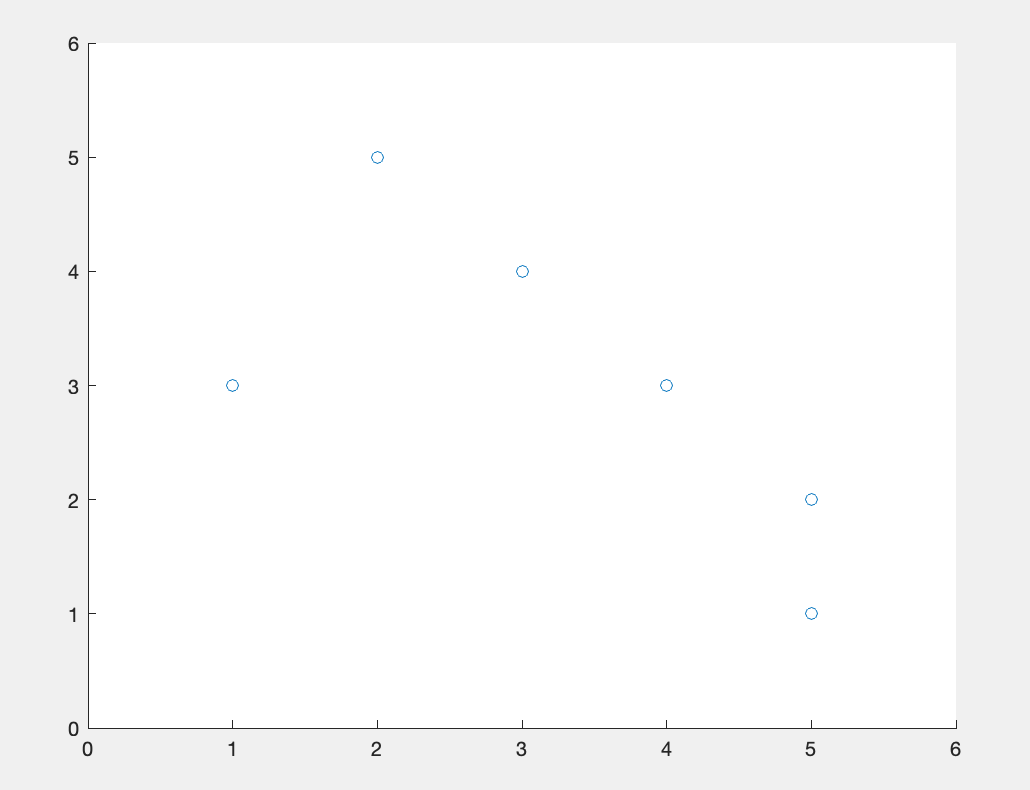
\includegraphics[scale=.6]{plot}\\
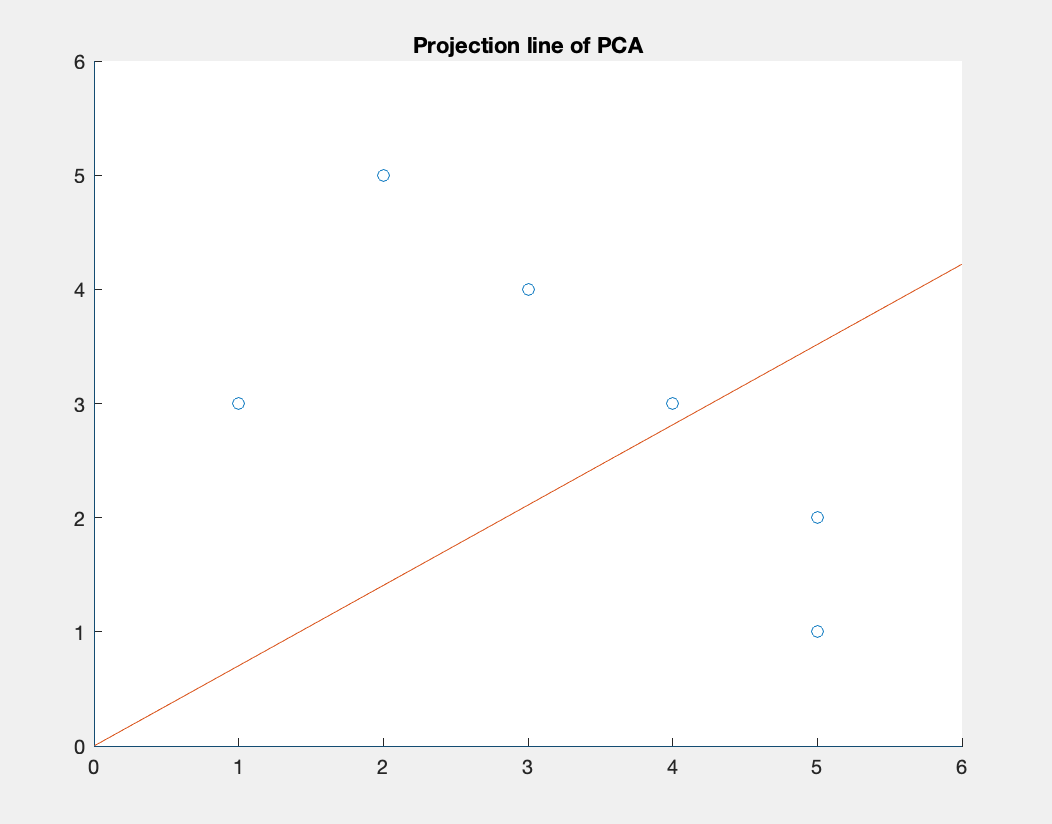
\includegraphics[scale=.6]{pca}\\
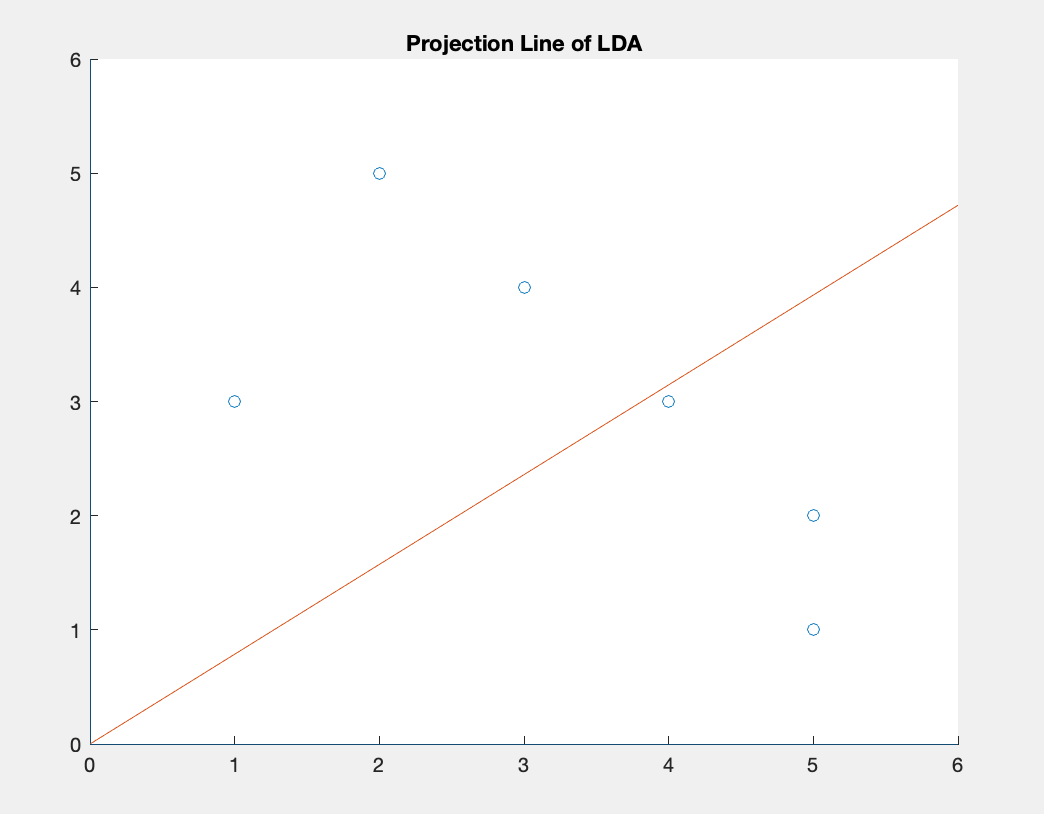
\includegraphics[scale=.6]{lda}

%Consider Non-negative Matrix Factorization Problem: $\minimize \limits_{\bm{\mA, \ \mG \geq 0}} \frac{1}{2}\|\mX-\mA\mG\|_F^2$.
%\begin{enumerate}
%	\item Please show that by leveraging gradient descent method with specific element-wise learning rate in each iteration, we will have:
%	\begin{equation}\label{mua}
%	\begin{aligned}
%	\mA_{k+1}&=\mA_k\odot\frac{\mX\mG_k^T}{\mA_k\mG_k\mG_k^T}\\
%	\mG_{k+1}&=\mG_k\odot\frac{\mA_{k+1}^T\mX}{\mA_{k+1}^T\mA_{k+1}\mG_k}\\
%	\end{aligned}
%	\end{equation}
%	where we use $\mZ\odot\mY$, $\frac{\mZ}{\mY}$ to represent component-wise multiplication and division between the corresponding elements of $\mZ$ and $\mY$ respectively.
%	\item We say $\mA$ is the feature matrix, please use the given \textit{atnt} dataset to plot the 10 feature faces by using \textit{MUA} to obtain $\mA$ after 500 iterations with random initializations ($\mA_0,\mG_0$).
%\end{enumerate}
%\vspace{4cm}


\section*{Problem 2}
Given positive data-set $\{\{1,1\},\{2,2\},\{2,3\}\}$, as well as negative data-set $\{\{3,2\},\{3,3\},\{4,4\}\}$, please determine the decision boundary when leveraging $k$-NN where $k=1$ and $k=3$ respectively.\\
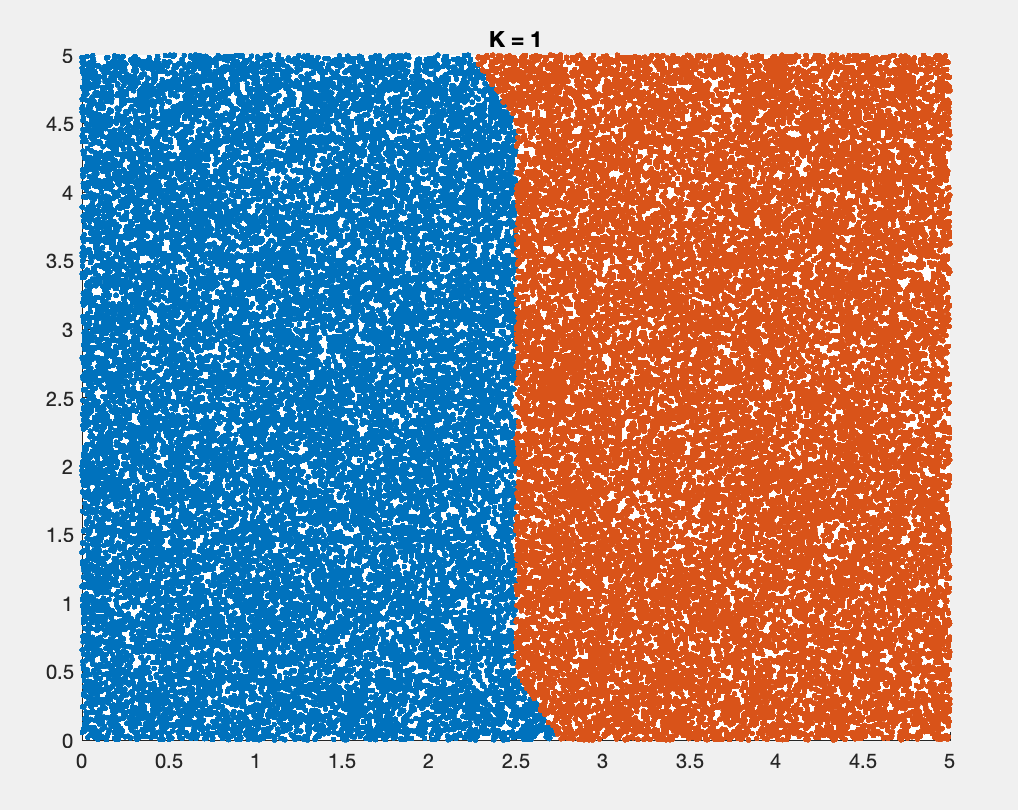
\includegraphics[scale=.6]{k=1}\\
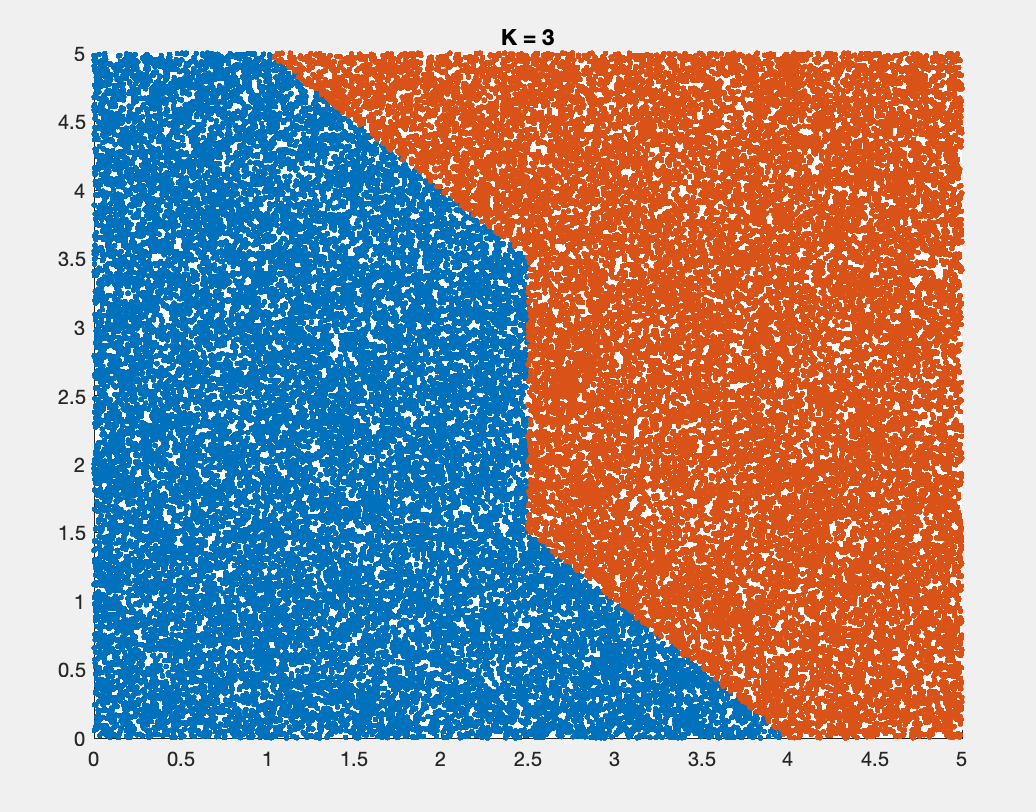
\includegraphics[scale=.6]{k=3}
%Please propose an alternating minimization method to update $\mA$ and $\mG$ column-by-column with close solution: $\minimize \limits_{\bm{\mA, \ \mG \geq 0}} \frac{1}{2}\|\mX-\mA\mG^T\|_F^2$. Then write a program to demonstrate that the objective is monotonically non-increasing with updates (certain figure is expected).

%\section*{Problem 3}
%Considering soft margin SVM, where we have the objective and constraints as follows:
%	\begin{equation}\label{eq:1}
%\begin{aligned}
%min\;\; &\frac{1}{2}||w||_2^2 +C\sum\limits_{i=1}^{m}\xi_i\\s.t.  \;\; y_i(w^Tx_i + &b)  \geq 1 - \xi_i \;\;(i =1,2,...m)\\\xi_i \geq &0 \;\;(i =1,2,...m)
%\end{aligned}
%\end{equation}
%Now we formulate another formulation as:
%	\begin{equation}
%\begin{aligned}
%min\;\; &\frac{1}{2}||w||_2^2 +\frac{C}{2}\sum\limits_{i=1}^{m}\xi_i^2\\s.t.  \;\; y_i(w^Tx_i + &b)  \geq 1 - \xi_i \;\;(i =1,2,...m)
%\end{aligned}
%\end{equation}
%\begin{enumerate}
%	\item Different from Eq. (\ref{eq:1}), we now drop the non-negative constraint for $\xi_i$, please show that optimal value of the objective will be the same when $\xi_i$ constraint is removed.\\
%	\answer{$\xi_i$ can't be negative, that is assume it is negative, then the constraint $y_i(w^Tx_i + b)  \geq 1 - \xi_i$ also satisifies for $\xi_i=0$ while the objective function would be lower.}
%	\item What's the generized Lagrangian of the new soft margin SVM optimization problem?\\
%	\answer{$\frac{1}{2}||w||_2^2 +\frac{C}{2}\sum\limits_{i=1}^{m}\xi_i^2-\sum\limits_{i=1}^{m}\alpha_i[y_i(w^Tx_i + b)- 1 + \xi_i]$, where $\alpha_i\geq0 \ (i =1,2,...m)$.}
%	\item Now please minimize the Lagrangian with respect to $w, b$, and $\xi$.\\
%	\answer{$w=\sum\limits_{i=1}^{m}\alpha_iy_ix_i, \ \sum\limits_{i=1}^{m}\alpha_iy_i=0, \ C\xi_i=\alpha_i \ (i =1,2,...m)$}
%	\item What is the dual of this version soft margin SVM optimization problem? (should be similar to Eq. (10) in the slides)\\
%	\answer{	\begin{equation}
%		\begin{aligned}
%		\underbrace{min}_{\alpha} \frac{1}{2}\sum\limits_{i=1}^{m}&\sum\limits_{j=1}^{m}\alpha_i\alpha_jy_iy_j \lg x_i, x_j\rg -  \sum\limits_{i=1}^{m} \alpha_i+\frac{1}{2C}\sum\limits_{i=1}^{m}\alpha_i^2\\&s.t. \; \sum\limits_{i=1}^{m}\alpha_iy_i = 0\\&\alpha_i \geq 0  \; i=1,2,...m
%		\end{aligned}
%		\end{equation}}
%	\item Please analysis bias-variance tradeoff when $C$ increases.\\
%	\answer{When $C$ increases, the bias decreases and variance increases since it is less tolerant with misclassification, thus the margin decreases, the generalization ability decreases.}
%	%\item Please show that 
%\end{enumerate}
%Let's revisit Least Squares Problem: $\minimize \limits_{\bm{\beta}} \frac{1}{2}\|\vy-\mA\bm{\beta}\|^2_2$, where $\mA\in\R^{n\times p}$.
%\begin{enumerate}
%	\item Please show that if $p>n$, then vanilla solution $(\mA^T\mA)^{-1}\mA^T\vy$ is not applicable any more.
%	\item Let's assume $\mA=[1, 2, 4;1, 3, 5; 1, 7, 7; 1, 8, 9], \vy=[1;2;3;4]$. Please show via experiment results that Gradient Descent method will obtain the optimal solution with  Linear Convergence rate if the learning rate is fixed to be $\frac{1}{\sigma_{max}(\mA^T\mA)}$, and $\bm{\beta}_0=[0;0;0]$.
%	\item Now let's consider ridge regression: $\minimize \limits_{\bm{\beta}} \frac{1}{2}\|\vy-\mA\bm{\beta}\|^2_2+\frac{\lambda}{2} \|\bm{\beta}\|^2_2$, where  $\mA,\vy,\bm{\beta}_0$ remains the same as above while learning rate is fixed to be $\frac{1}{\lambda+\sigma_{max}(\mA^T\mA)}$ where $\lambda$ varies from $0.1,1,10,100,200$, please show that Gradient Descent method with larger $\lambda$ converges faster. (You will receive up to 10 bonus points if you can prove faster convergence rate mathematically.)
%\end{enumerate}

%\vspace{1cm}
%\section*{Problem 4}
%Please download the image from \url{https://en.wikipedia.org/wiki/Lenna#/media/File:Lenna_(test_image).png} with dimension $512\times512\times3$. Assume for each RGB channel data $X$, we have $[U,\Sigma,V]=svd(X)$. Please show each compression ratio and reconstruction image if we choose first $2, 5, 20, 50,80,100$ components respectively. Also  please determine the best component number to obtain a good trade-off between data compression ratio and reconstruction image quality. (Open question, that is your solution will be accepted as long as it's reasonable.)
%
%\vspace{1cm}
%\section*{Problem 5}
% Draw the first two principle components for the following dataset.
% \begin{figure}[h!]
% 	\centering
% 	\includegraphics[width=.5\linewidth]{robustPCA}
% \end{figure}
%Based on this, comment on a limitation of PCA and think about how to improve it.\\

\section*{Problem 3}
Given $X, Y, Z$, now please follow the idea/method used in LDA/PCA to find the best solution to:
\begin{equation}
\begin{aligned}
&\underbrace{arg\;max}_{a,b}\;\;{a^TZb}\\
s.t. \ \ &a^TXa =1,\; b^TYb =1
\end{aligned}
\end{equation}
Since $X, Y, Z$ are SPD we can expand our constraints $s.t.$ $ a^TX^{1/2}X^{1/2}a = 1, $ $b^TY^{1/2}Y^{1/2}b = 1$\\\\
Let $u$ = $X^{1/2}a$ and $v$ = $Y^{1/2}b$, therefore we have that $u^Tu = 1$ and $v^Tv = 1$\\\\We can arrange to say that $a^T = u^TX^{1/2}$ and $b = Y^{1/2}v$ and therefore we $max$ $u^TX^{-1/2}ZY^{-1/2}v$\\\\If we use SVD we find that $[U, \Sigma, V] = svd(X^{-1/2}ZY^{-1/2})$. We can then let $u$ be the first column of $U$, and $v$ be the first column of $V$, and then find a and b.

\section*{Code}
NOTE: For plotting data points on graph I just removed some aspects of the PCA projection code.\\
\textbf{PCA Projection Line Code}\\
\lstinputlisting{pca_projection.m}
\textbf{LDA Projection Line}\\
\lstinputlisting{lda_projection.m}
\textbf{LDA Algorithm}\\
\lstinputlisting{LDA.m}
\textbf{KNN Boundary Code}\\
\lstinputlisting{knn_boundary.m}
\textbf{KNN Algorithm}\\
\lstinputlisting{KNN.m}


\end{document}

